% Set parameters
% set font size
\documentclass[11pt]{article}

% set line height
\renewcommand{\baselinestretch}{1.5}

% line number
\usepackage{lineno}

% today
\renewcommand{\today}{}

% set margin
\usepackage{geometry}
\geometry{a4paper, left=15mm, right=15mm, top=20mm, bottom=20mm}

% for using Korean
\usepackage{kotex}

% for using multi-languages
\usepackage[english]{babel}

% for urls
\usepackage{hyperref}

% for equation
\usepackage{amsmath}

% for bibliography
\usepackage{apacite}
\usepackage[numbers]{natbib}

% for drawing table
\usepackage{array,multirow,graphicx,rotating,booktabs}
\usepackage[table,xcdraw]{xcolor}

% for tabularx
\usepackage{tabularx}
\newcolumntype{b}{X}
\newcolumntype{s}{>{\hsize=.5\hsize}X}
\renewcommand\arraystretch{0.8} \setlength\minrowclearance{0.8pt}

%%%%%%%%%%%%%%%%%%%%%%%%%%%%%%%%%%%%%%%%%%%%%%%%%%%%%%%%%%%%%%%%%%%%%%%%%%%%%%%
\begin{document}

\title{Title example}
\author{
  Hyunjoong Kim\\
  \texttt{soy.lovit@gmail.com}
  \and
  Lovit\\
  \texttt{soy.lovit@gmail.com}
}

\maketitle
\smallskip

%%%%%%%%%%%%%%%%%%%%%%%%%%%%%%%%%%%%%%%%%%%%%%%%%%%%%%%%%%%%%%%%%%%%%%%%%%%%%%%
\section{Introduction}

인트로의 내용은 한 문장을 한 줄로 쓰라는 것입니다.
이유는 git commit log 를 보시면 알 수 있습니다.
다음 줄로 넘어가도 하나의 단락 안에 포함됩니다.
한 문장을 한줄에 넣으면 이후 git 으로 latex 코드를 관리할 때, 수정한 줄을 확인할 수 있습니다.

빈 줄을 하나 이상 추가하면 다음 단락으로 만들어집니다.

\noindent
들여쓰기를 하지 않으려면 noindent 를 입력합니다.

다음 단락은 들여쓰기가 다시 됩니다.

%%%%%%%%%%%%%%%%%%%%%%%%%%%%%%%%%%%%%%%%%%%%%%%%%%%%%%%%%%%%%%%%%%%%%%%%%%%%%%%
\section{git commit 을 통한 버전 관리}

위의 introduction section 의 내용을 수정 한 뒤, github 에 commit 을 했습니다.
각 commit 마다 comment 를 달 수 있습니다.
짧은 내용에 대한 논의 및 메모는 이를 통하여 할 수 있습니다.

\begin{figure}[ht]
\centering
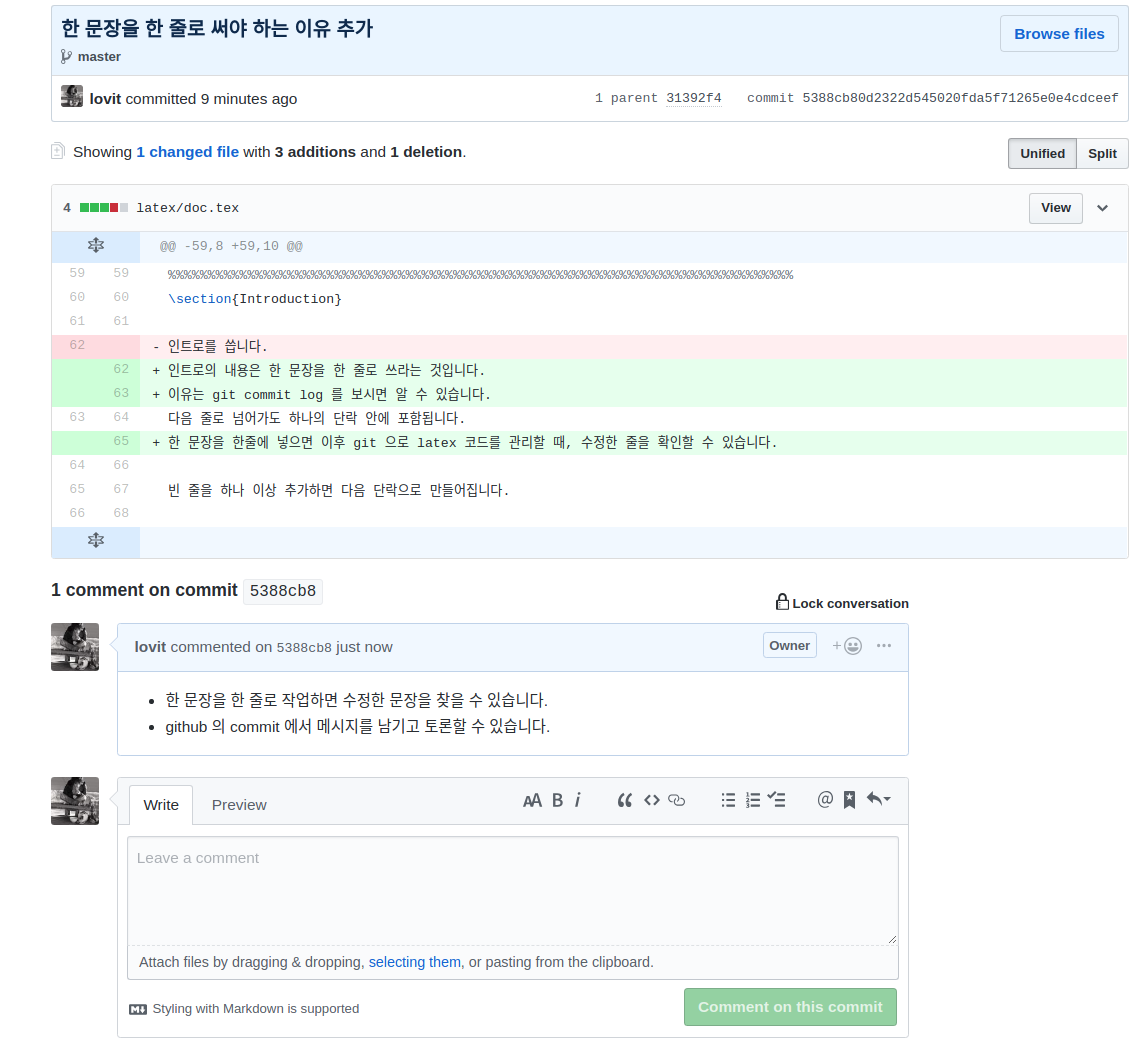
\includegraphics[keepaspectratio=true, width=0.8\linewidth]{figures/git-commit-comment.png}
\caption{github commit 에 comment 를 달아둔 snapshot}
\label{fig:commit_comment}
\end{figure}

그림 \ref{fig:commit_comment} 을 보면 한 문장을 한 줄로 작성했기 때문에 변화한 문장을 찾을 수 있습니다.
한 줄의 코드에 여러 문장이 포함되어 있으면 하이라이팅이 제대로 되지 않을 때가 있습니다.

%%%%%%%%%%%%%%%%%%%%%%%%%%%%%%%%%%%%%%%%%%%%%%%%%%%%%%%%%%%%%%%%%%%%%%%%%%%%%%%
\subsection{Branch 로 주제 단위 별 commit 관리하기}

동시에 여러 section 을 작업할 때도 있습니다.
혹은 여러 명이 부분을 맡아서 작업하기도 합니다.
이 때 각 일의 단위 별로 branch 를 만들어 수정 작업을 하면 그 단위 별로 commit log 가 정리되어 보입니다.
최종 수정본은 master branch 로 merging 합니다.

\begin{figure}[ht]
\centering
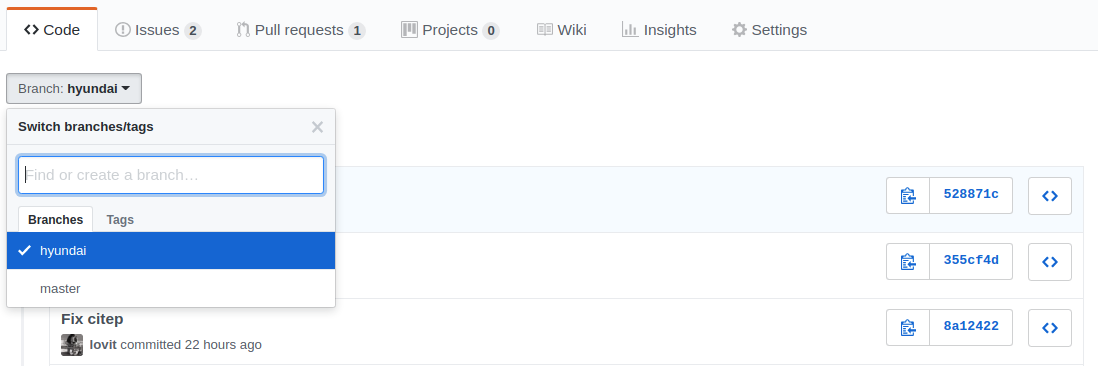
\includegraphics[keepaspectratio=true, width=0.8\linewidth]{figures/github-branch.png}
\caption{github commit 에 comment 를 달아둔 snapshot}
\label{fig:github-issue}
\end{figure}

%%%%%%%%%%%%%%%%%%%%%%%%%%%%%%%%%%%%%%%%%%%%%%%%%%%%%%%%%%%%%%%%%%%%%%%%%%%%%%%
\subsection{Issue 를 이용하여 todo list 관리하기}

협업을 할 때 todo 를 적어두기도 합니다.
수정해야 하는 부분이 있고, 이를 누군가에게 assign 할 일도 있다면 github issue board 를 이용할 수 있습니다.
github 의 issue 에 해야 할 일을 적어두고, 해결된 뒤에는 issue 를 close 합니다.

\begin{figure}[ht]
\centering
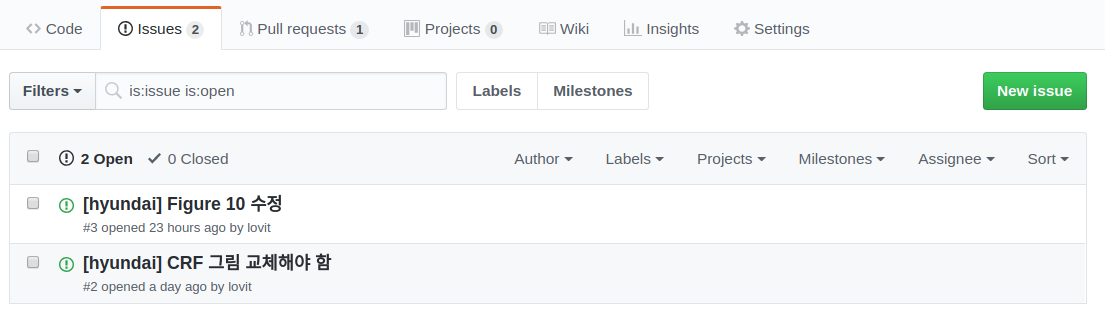
\includegraphics[keepaspectratio=true, width=0.8\linewidth]{figures/github-issue.png}
\caption{github commit 에 comment 를 달아둔 snapshot}
\label{fig:github-issue}
\end{figure}

%%%%%%%%%%%%%%%%%%%%%%%%%%%%%%%%%%%%%%%%%%%%%%%%%%%%%%%%%%%%%%%%%%%%%%%%%%%%%%%
\subsection{목차 단위}

section 을 입력하면 1, 2, 3 장 이 됩니다.

subsection 을 입력하면 1.1, 1.2, ... 2.1 장이 됩니다. section 의 번호를 따라갑니다.

%%%%%%%%%%%%%%%%%%%%%%%%%%%%%%%%%%%%%%%%%%%%%%%%%%%%%%%%%%%%%%%%%%%%%%%%%%%%%%%
\section{두번째 장}

코드의 가독성을 위하여 section 마다 주석코드인 \% 를 나열하면 좋습니다.

\section{Reference 달기}

citep 를 이용합니다. bib 파일에 있는 idx 를 citep 에 넣습니다. \citep{jain2010data} 대괄호 안에 여러 개의 idx 를 , 로 연결할 수 있습니다.

%%%%%%%%%%%%%%%%%%%%%%%%%%%%%%%%%%%%%%%%%%%%%%%%%%%%%%%%%%%%%%%%%%%%%%%%%%%%%%%
\section{Equation}

수식 영역도 begin, end 로 지정합니다.
centering 은 가운데 정렬을 도와줍니다.
수식, 그림, 표를 다른 곳에서 호출하기 위해서는 label 을 지정해줍니다.
equation 형식이라는 의미로 eq, 이 함수의 이름은 kpartition 이라 정의합니다.

\begin{equation}
\label{eq:kpartition}
\centering
arg min_C\sum_{i=1}^{k} \sum_{x \in C_i} \vert x - \mu_i \vert^2 = arg min_C \sum_{i=1}^{k} \vert C_i \vert Var(C_i)
\end{equation}

지정된 수식은 ref 를 이용하여 링크를 걸 수 있습니다 (수식 \ref{eq:kpartition})

%%%%%%%%%%%%%%%%%%%%%%%%%%%%%%%%%%%%%%%%%%%%%%%%%%%%%%%%%%%%%%%%%%%%%%%%%%%%%%%
\section{표 만들기}

표를 만들기 위해서는 직접 코드를 짜도 좋지만, online table generator \footnote{\url{https://www.tablesgenerator.com/latex_tables}} 를 이용할 수도 있습니다. 
이 사이트에서는 csv 파일을 읽어서 이를 표로 만들어주기도 합니다.

%%%%%%%%%%%%%%%%%%%%%%%%%%%%%%%%%%%%%%%%%%%%%%%%%%%%%%%%%%%%%%%%%%%%%%%%%%%%%%%
\section{그림 참조}

만들어진 그림도 링크를 걸 수 있습니다. (그림 \ref{fig:community_detection})

\begin{figure}[ht]
\centering
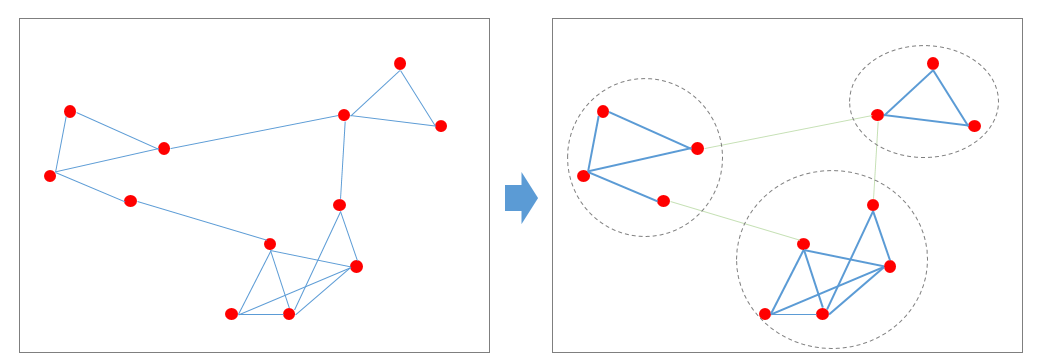
\includegraphics[keepaspectratio=true, width=0.5\linewidth]{figures/community_detection.png}
\caption{caption 에 텍스트를 넣습니다.}
\label{fig:community_detection}
\end{figure}

%%%%%%%%%%%%%%%%%%%%%%%%%%%%%%%%%%%%%%%%%%%%%%%%%%%%%%%%%%%%%%%%%%%%%%%%%%%%%%%
\section{bib 파일 관리}

bib 파일은 reference 들의 제목, 저자, 연도, 출판사, 저널 및 학회 이름 등을 저장해둔 파일입니다.
google 에서 검색하면 저널 들에 citation 메뉴가 있습니다.
이를 클릭하여 BibTex 를 누르면 bib 형식으로 reference 를 보여줍니다.
하나의 reference 를 한 줄로 적기 위해 줄바꿈을 제거하여 bib 에 넣는 것을 선호합니다.

%%%%%%%%%%%%%%%%%%%%%%%%%%%%%%%%%%%%%%%%%%%%%%%%%%%%%%%%%%%%%%%%%%%%%%%%%%%%%%%
\section{Latex to pdf}

Latex compiler 를 이용해도 됩니다.
하지만 latex 설치를 하고 싶지 않다면, (그 과정에서 겪는 어려움을 피하고 싶다면) overleaf.com 과 같은 온라인 서비스를 이용할 수도 있습니다.

pdf 파일은 byte 이기 때문에 수정된 부분만 tracking 이 되지 않습니다.
git 에 pdf 를 추가할 때에는 최종본, 혹은 중간에 저장을 해둬야 하는 파일만 합니다.

%%%%%%%%%%%%%%%%%%%%%%%%%%%%%%%%%%%%%%%%%%%%%%%%%%%%%%%%%%%%%%%%%%%%%%%%%%%%%%%
%\bibliographystyle{unsrtnat}
\bibliographystyle{apacite}
\bibliography{reference}

%%%%%%%%%%%%%%%%%%%%%%%%%%%%%%%%%%%%%%%%%%%%%%%%%%%%%%%%%%%%%%%%%%%%%%%%%%%%%%%
\section*{Appendix}

section* 를 이용하면 번호가 붙지 않는 section 이 만들어집니다.

\end{document}
